% latex trie1.tex
% dvisvgm --no-fonts --exact --bbox=papersize --output=trie1.svg trie1.dvi
\documentclass[tikz,border=6pt]{standalone}
\usetikzlibrary{arrows.meta}
\begin{document}
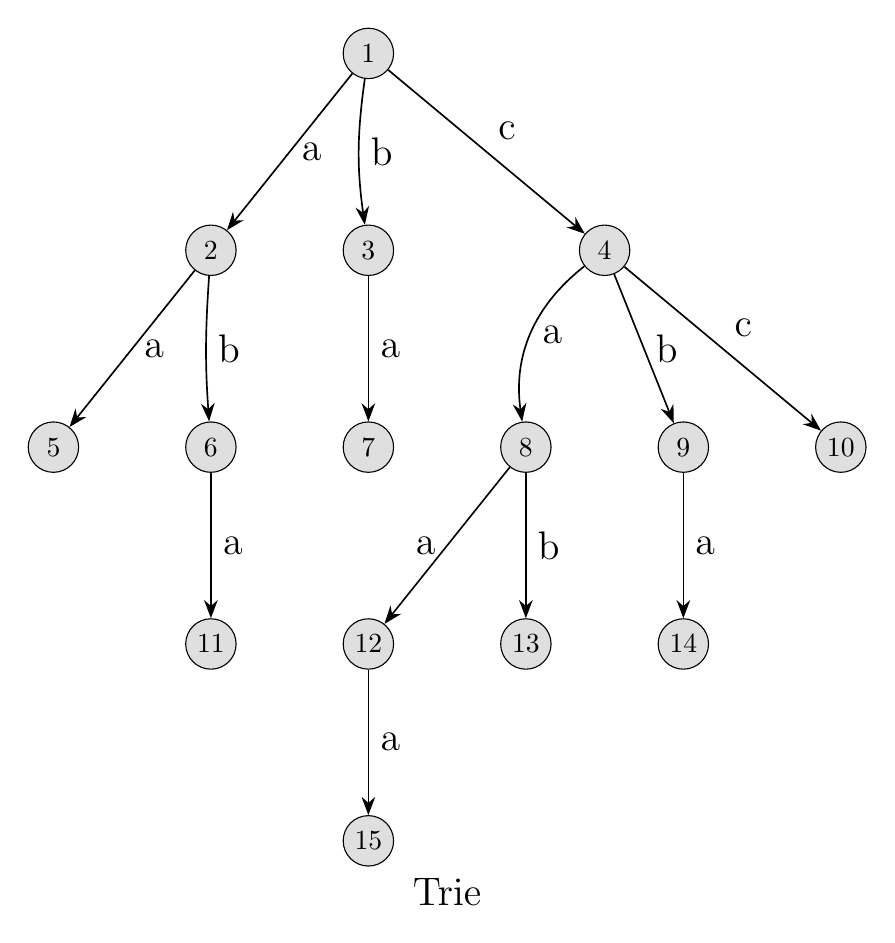
\begin{tikzpicture}[
    state/.style={circle,draw,fill=gray!25,minimum size=0.64cm,inner sep=0pt},
    edge/.style={-{Stealth[length=2.3mm]},line width=0.6pt},
    label/.style={font=\Large,inner sep=4pt}
  ]
  \foreach \id/\x/\y in {
      1/4/0,
      2/2/-2.5,3/4/-2.5,4/7/-2.5,
      5/0/-5,6/2/-5,7/4/-5,8/6/-5,9/8/-5,10/10/-5,
      11/2/-7.5,12/4/-7.5,13/6/-7.5,14/8/-7.5,
      15/4/-10} {
    \node[state] (n\id) at (\x,\y) {\id};
  }
  % Edge labels spell the strings represented by paths from the root.
  \draw[edge] (n1) -- node[label,right] {a} (n2);
  \draw[edge] (n1) to[bend right=8] node[label,right] {b} (n3);
  \draw[edge] (n1) -- node[label,above right] {c} (n4);
  \draw[edge] (n2) -- node[label,right] {a} (n5);
  \draw[edge] (n2) to[bend right=4] node[label,right] {b} (n6);
  \draw[edge] (n3) -- node[label,right] {a} (n7);
  \draw[edge] (n4) to[bend right=30] node[label,right] {a} (n8);
  \draw[edge] (n4) -- node[label,right] {b} (n9);
  \draw[edge] (n4) -- node[label,above right] {c} (n10);
  \draw[edge] (n6) -- node[label,right] {a} (n11);
  \draw[edge] (n8) -- node[label,left] {a} (n12);
  \draw[edge] (n8) -- node[label,right] {b} (n13);
  \draw[edge] (n9) -- node[label,right] {a} (n14);
  \draw[edge] (n12) -- node[label,right] {a} (n15);
  \node[font=\Large] at (5,-10.65) {Trie};
\end{tikzpicture}
\end{document}
